% Choose one to switch between slides and handout
%\documentclass[]{beamer}
\documentclass[handout]{beamer}

% Video Meta Data
\title{Bitcoin, Blockchain and Cryptoassets}
\subtitle{SegWit and Transaction Malleability}
\author{Prof. Dr. Fabian Schär}
\institute{University of Basel}

% Config File
% Packages
\usepackage[utf8]{inputenc}
\usepackage{hyperref}
\usepackage{gitinfo2}
\usepackage{tikz}
\usepackage{amsmath}
\usepackage{mathtools}
\usepackage{bibentry}
\usepackage{xcolor}
\usepackage{colortbl} % Add colour to LaTeX tables
\usepackage{caption}
\usepackage[export]{adjustbox}
\usepackage{pgfplots} \pgfplotsset{compat = 1.17}
\usepackage{makecell}
\usepackage{fancybox}
\usepackage{ragged2e}
\usepackage{fontawesome}
\usepackage{seqsplit}
\usepackage{tabularx}

% Color Options
\definecolor{highlight}{rgb}{0.65,0.84,0.82}
\definecolor{focus}{rgb}{0.72, 0, 0}
\definecolor{lightred}{rgb}{0.8,0.5,0.5}
\definecolor{midgray}{RGB}{190,195,200}

% Beamer Template Options
\beamertemplatenavigationsymbolsempty
\setbeamertemplate{footline}[frame number]
\setbeamercolor{structure}{fg=black}
\setbeamercolor{footline}{fg=black}
\setbeamercolor{title}{fg=black}
\setbeamercolor{frametitle}{fg=black}
\setbeamercolor{item}{fg=black}
\setbeamercolor{}{fg=black}
\setbeamercolor{bibliography item}{fg=black}
\setbeamercolor*{bibliography entry title}{fg=black}
\setbeamercolor{alerted text}{fg=focus}
\setbeamertemplate{items}[square]
\setbeamertemplate{enumerate items}[default]
\captionsetup[figure]{labelfont={color=black},font={color=black}}
\captionsetup[table]{labelfont={color=black},font={color=black}}

\setbeamertemplate{bibliography item}{\insertbiblabel}

% Link Icon Command
\newcommand{\link}{%
    \tikz[x=1.2ex, y=1.2ex, baseline=-0.05ex]{%
        \begin{scope}[x=1ex, y=1ex]
            \clip (-0.1,-0.1)
                --++ (-0, 1.2)
                --++ (0.6, 0)
                --++ (0, -0.6)
                --++ (0.6, 0)
                --++ (0, -1);
            \path[draw,
                line width = 0.5,
                rounded corners=0.5]
                (0,0) rectangle (1,1);
        \end{scope}
        \path[draw, line width = 0.5] (0.5, 0.5)
            -- (1, 1);
        \path[draw, line width = 0.5] (0.6, 1)
            -- (1, 1) -- (1, 0.6);
        }
    }

% Read Git Data from Github Actions Workflow
% Defaults to gitinfo2 for local builds
\IfFileExists{gitInfo.txt}
	{\input{gitInfo.txt}}
	{
		\newcommand{\gitRelease}{(Local Release)}
		\newcommand{\gitSHA}{\gitHash}
		\newcommand{\gitDate}{\gitAuthorIsoDate}
	}

% Custom Titlepage
\defbeamertemplate*{title page}{customized}[1][]
{
  \vspace{-0cm}\hfill\includegraphics[width=2.5cm]{../config/logo_cif}
  \includegraphics[width=1.9cm]{../config/seal_wwz}
  \\ \vspace{2em}
  \usebeamerfont{title}\textbf{\inserttitle}\par
  \usebeamerfont{title}\usebeamercolor[fg]{title}\insertsubtitle\par  \vspace{1.5em}
  \small\usebeamerfont{author}\insertauthor\par
  \usebeamerfont{author}\insertinstitute\par \vspace{2em}
  \usebeamercolor[fg]{titlegraphic}\inserttitlegraphic
    \tiny \noindent \texttt{Release Ver.: \gitRelease}\\ 
    \texttt{Version Hash: \gitSHA}\\
    \texttt{Version Date: \gitDate}\\ \vspace{1em}
    
    
    \iffalse
  \link \href{https://github.com/cifunibas/Bitcoin-Blockchain-Cryptoassets/blob/main/slides/intro.pdf}
  {Get most recent version}\\
  \link \href{https://github.com/cifunibas/Bitcoin-Blockchain-Cryptoassets/blob/main/slides/intro.pdf}
  {Watch video lecture}\\ 
  
  \fi
  
  \vspace{1em}
  License: \texttt{Creative Commons Attribution-NonCommercial-ShareAlike 4.0 International}\\\vspace{2em}
  \includegraphics[width = 1.2cm]{../config/license}
}


% tikzlibraries
\usetikzlibrary{decorations.pathreplacing}
\usetikzlibrary{decorations.markings}
\usetikzlibrary{positioning}
\usetikzlibrary{calc}
\captionsetup{font=footnotesize}


%%%%%%%%%%%%%%%%%%%%%%%%%%%%%%%%%%%%%%%%%%%%%%
%%%%%%%%%%%%%%%%%%%%%%%%%%%%%%%%%%%%%%%%%%%%%%
\begin{document}

\thispagestyle{empty}
\begin{frame}[noframenumbering]
	\titlepage
\end{frame}

%%%
\begin{frame}{Transaction Structure}

\begin{figure}
	 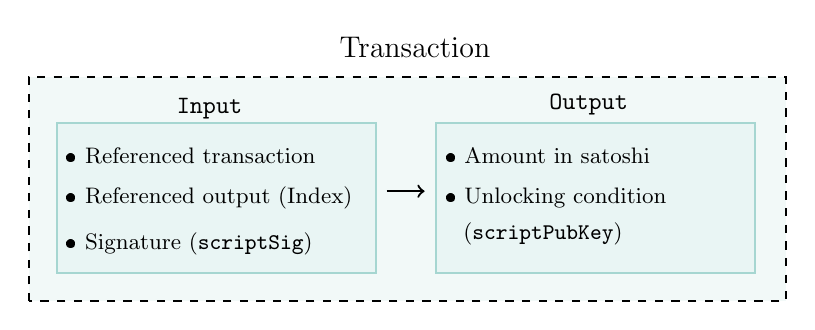
\begin{tikzpicture}[scale=0.9, every node/.style={scale=0.9}]
    
        \filldraw[yshift=-0.05cm, xshift=0.1cm,color = highlight!15, thick, draw=black, dashed] (-4,-4) rectangle ++(304pt,90pt) ;
    
        \filldraw[yshift=-0.05cm, xshift=0.1cm,color = highlight!25, thick, draw=highlight] (-3.6,-3.6) rectangle ++(128pt,60pt) ;
    
    \draw[->,thick] (1.15,-2.5) -- (1.685,-2.5) ;
    
    \draw[color=black] plot (-1.35,-1.6)   node[above] {\texttt{Input}};
    \draw[color=black] plot (-3.5,-2)   node[right] {\small{\textbullet{} {Referenced transaction}}};
    \draw[color=black] plot (-3.5,-2.6)   node[right] {\small{\textbullet{} Referenced output (Index)}};
    \draw[color=black] plot (-3.5,-3.25)   node[right] {\small{\textbullet{} Signature (\texttt{scriptSig})}};
    \draw[color=black] plot (1.55,-0.2) node [below]
    {\large{{Transaction}}};
    
    
        \filldraw[yshift=-0.05cm, xshift=0.1cm,color = highlight!25, thick, draw=highlight] (1.75,-3.6) rectangle ++(128pt,60pt) ;
    
    \draw[color=black] plot (4,-1.55)   node[above] {\texttt{Output}};
    \draw[color=black] plot (1.85,-2)   node[right] {\small{\textbullet{} Amount in satoshi}};
    \draw[color=black] plot (1.85,-2.6)   node[right] {\small{\textbullet{} Unlocking condition}};
    \draw[color=black] plot (2,-3.1)   node[right] {\small{ (\texttt{scriptPubKey})}};
    %\draw[color=black] plot (1.95,-3.2)   node[right] {\small{\textbullet{} Signatur / Lösung}};
    
    \end{tikzpicture}
	
\end{figure}
\vspace{1em}

\uncover<2->{$\rightarrow$ The \texttt{scriptSig} is part of the transaction data and cannot be signed (self-referential).}

\end{frame}
%%%

%%%
\begin{frame}{Transaction Malleability}

Typical transaction data:\\
\begin{scriptsize}
	\texttt{\textcolor{black!30}{0100000001c997a5e56e104102fa209c6a852dd90660a20b2d9c352423edce25857fcd3704
		00000000}{\alert{4847304402204e45e16932b8af514961a1d3a1a25fdf3f4f7732e9d624c6c61548
		ab5fb8cd410220181522ec8eca07de4860a4acdd12909d831cc56cbbac4622082221a8768d
		1d0901}}\textcolor{black!30}{ffffffff0200ca9a3b00000000434104ae1a62fe09c5f51b13905f07f06b99a2f715
		9b2225f374cd378d71302fa28414e7aab37397f554a7df5f142c21c1b7303b8a0626f1bade
		d5c72a704f7e6cd84cac00286bee0000000043410411db93e1dcdb8a016b49840f8c53bc1e
		b68a382e97b1482ecad7b148a6909a5cb2e0eaddfb84ccf9744464f82e160bfa9b8b64f9d4
		c03f999b8643f656b412a3ac00000000}}
\end{scriptsize}
	\vspace{1em}
	
	\uncover<2->{This transaction data hashes to the following TXID:\\
		\begin{scriptsize}
			\texttt{f4184fc596403b9d638783cf57adfe4c75c605f6356fbc91338530e9831e9e16}
		\end{scriptsize}
	\vspace{1em}
	
	\uncover<3->{$\rightarrow$ But anyone can change the \alert{\texttt{scriptSig}} without invalidating the transaction. The TXID is not a reliable transaction identifier.}
	}
\end{frame}
%%%

%%%
\begin{frame}{Signature-Based Malleability Sources}

	The cryptographic signature is part of the \texttt{scriptSig}:\\
	
	\begin{scriptsize}
		\begin{figure}
			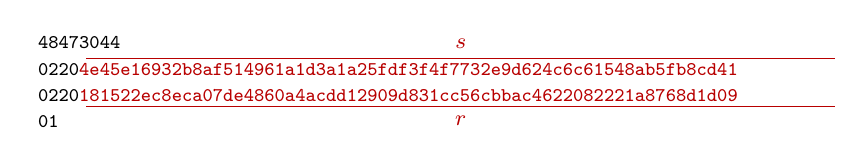
\begin{tikzpicture}[scale = 0.67]

	\draw 			(0,1.5) node [right] {\scriptsize \texttt{48473044}};


	\draw 			(0,1) node [right] {\scriptsize \texttt{0220\textcolor{focus}{4e45e16932b8af514961a1d3a1a25fdf3f4f7732e9d624c6c61548ab5fb8cd41}}};
	
	\draw 			(0,0.5) node [right] {\scriptsize \texttt{0220\textcolor{focus}{181522ec8eca07de4860a4acdd12909d831cc56cbbac4622082221a8768d1d09}}};
	
	\draw 			(0,0) node [right] {\scriptsize \texttt{01}};
		
	\draw [focus] 	(1.1,1.2) node [left]{} --
					(15.3,1.2) node [midway,above] {\footnotesize \color{focus} $s$};
										
	\draw [focus] 	(1.1,0.3) node [left]{} --
					(15.3,0.3) node [midway,below] {\footnotesize \color{focus} $r$};					
	
\end{tikzpicture}

		\end{figure}
	\end{scriptsize}
	
	Two signature-based malleability sources:
	\begin{itemize}
		\item[1.] OpenSSL allows for $r$ and $s$ to be encoded in a variety of ways.
		\item<2-> [2.] Using the negative of $s$ does not invalidate the signature.
	\end{itemize}
	
	\uncover<3->{
		\begin{scriptsize}
			From the \href{https://cryptolectures.teachable.com/courses/bitcoin-blockchain-and-cryptoassets/lectures/30728675}{\link ECDSA example}; assume an attacker changes $s$ from 7 to -7:\\
			\vspace{-0.5em}
			\begin{columns}[T]
				\begin{column}{0.5\textwidth}
					\begin{align*}
						\uncover<3->{
						(-s^{-1})\ mod\ n &= (-7^{-1})\ mod\ 13\\
										&= 11 \\
						\text{since:}\ (-7^{-1} \cdot 11)\ mod\ 13 &= 1\\
						}
						\vspace{0.5em}
						\uncover<4->{
							u_1 &= (-s^{-1}t)\ mod\ n\\
								&= (11 \cdot 4)\ mod\ 13\\
								&= 5\\
						}
						\vspace{0.5em}
						\uncover<5->{
							u_2 &= (-s^{-1}r)\ mod\ n\\
								&= (11 \cdot 5)\ mod\ 13\\
								&= 3\\
						}
					\end{align*}
				\end{column}
				\begin{column}{0.5\textwidth}
					\begin{align*}
						\uncover<6->{
							P 	&= u_1 \circ G + u_2 \circ K_{pub}\\
								&= 5 \circ (8,1) + 3 \circ (23,1)\\
								&= (32,17) + (8,1)\\
								&= (18,17)\\
						}
						\vspace{0.5em}
						\uncover<7->{
							x_P\ mod\ n &= 18\ mod\ 13\\
										&= 5\\
										&= r
						}
					\end{align*}
				\end{column}
			\end{columns}
		\end{scriptsize}
	}
\end{frame}
%%%

%%%
\begin{frame}{Operation Code-Based Malleability Sources}
	\begin{scriptsize}
		From the \href{https://cryptolectures.teachable.com/courses/bitcoin-blockchain-and-cryptoassets/lectures/30728695}{\link P2PK example}:
	\end{scriptsize}
	\begin{itemize}
		\item<1->[1.] \texttt{OP\_PUSHDATA 47}
		\item<2->[2.] \texttt{OP\_PUSHDATA 41}
	\end{itemize}
	\vspace{1em}

	\begin{figure}
		\begin{tikzpicture}[scale=1, every node/.style={scale=1.4}]  %,domain=0:8

\draw[very thick] (-0.1,0) -- (4.1,0);
\draw[very thick] (-0.1,0) -- (-0.1,4);
\draw[very thick] (4.1,0) -- (4.1,4);
\draw (2,-0.5) node[below] {\texttt{Stack}};

\only<1,2,5>{
\draw[color=white] plot (6.1,4.7)   node[minimum width=2.7cm, minimum height=0.55cm,fill=white, thick,  draw=white,below, rotate = 0] {\texttt{Dummy}};
}

\only<5>{
\draw[color=black] plot (2,0.8)   node[minimum width=2.9cm,fill=highlight!15, thick,  draw=highlight,below, rotate = 0] {\texttt{1}};
}

\only<1-3>{
\draw[color=black] plot (2,0.8)   node[minimum width=2.7cm,fill=highlight!15, thick, draw=highlight,below, rotate = 0] {\texttt{304402...0901}};
}

\only<2-3>{
\draw[color=black] plot (2,1.6)   node[minimum width=2.7cm, fill=focus!15, thick,  draw=focus,below, rotate = 0] {\texttt{0411db...12a3}};
}

\only<3-4>{
\draw[color=black] plot (6.1,4.7)   node[minimum width=2.7cm ,minimum height= 0.5cm, fill=black!15, thick,  draw=black,below, rotate = 0] {\texttt{ac}};
}

\only<4>{
\draw[color=black] plot (2,4.7)   node[minimum width=2.7cm,fill=focus!15, thick,  draw=focus,below, rotate = 0] {\texttt{0411db...12a3}};
}

\only<4>{
\draw[color=black] plot (2,3.9)   node[minimum width=2.7cm,fill=highlight!15, thick,  draw=highlight,below, rotate = 0] {\texttt{304402...0901}};
}

\end{tikzpicture}	
	\end{figure}
\end{frame}
%%%

%%%
\begin{frame}{Operation Code-Based Malleability Sources}
	Changing the script in a way which does not affect the stack:
	\begin{itemize}
		\item<1->[1.] \texttt{\alert{OP\_PUSHDATA2 0047}}
		\item<2->[2.] \texttt{OP\_PUSHDATA 41}
	\end{itemize}
	\vspace{1.5em}

	\begin{figure}
		\begin{tikzpicture}[scale=1, every node/.style={scale=1.4}]  %,domain=0:8

\draw[very thick] (-0.1,0) -- (4.1,0);
\draw[very thick] (-0.1,0) -- (-0.1,4);
\draw[very thick] (4.1,0) -- (4.1,4);
\draw (2,-0.5) node[below] {\texttt{Stack}};

\only<1,2,5>{
\draw[color=white] plot (6.1,4.7)   node[minimum width=2.7cm, minimum height=0.55cm,fill=white, thick,  draw=white,below, rotate = 0] {\texttt{Dummy}};
}

\only<5>{
\draw[color=black] plot (2,0.8)   node[minimum width=2.9cm,fill=highlight!15, thick,  draw=highlight,below, rotate = 0] {\texttt{1}};
}

\only<1-3>{
\draw[color=black] plot (2,0.8)   node[minimum width=2.7cm,fill=highlight!15, thick, draw=highlight,below, rotate = 0] {\texttt{304402...0901}};
}

\only<2-3>{
\draw[color=black] plot (2,1.6)   node[minimum width=2.7cm, fill=focus!15, thick,  draw=focus,below, rotate = 0] {\texttt{0411db...12a3}};
}

\only<3-4>{
\draw[color=black] plot (6.1,4.7)   node[minimum width=2.7cm ,minimum height= 0.5cm, fill=black!15, thick,  draw=black,below, rotate = 0] {\texttt{ac}};
}

\only<4>{
\draw[color=black] plot (2,4.7)   node[minimum width=2.7cm,fill=focus!15, thick,  draw=focus,below, rotate = 0] {\texttt{0411db...12a3}};
}

\only<4>{
\draw[color=black] plot (2,3.9)   node[minimum width=2.7cm,fill=highlight!15, thick,  draw=highlight,below, rotate = 0] {\texttt{304402...0901}};
}

\end{tikzpicture}	
	\end{figure}
\end{frame}
%%%

%%%
\begin{frame}{Operation Code-Based Malleability Sources}
From the previous transaction data:\\
\begin{scriptsize}
	\texttt{\textcolor{focus}{47}304402204e45e16932b8af514961a1d3a1a25fdf3f4f77
	32e9d624c6c61548ab5fb8cd410220181522ec8eca07de48
	60a4acdd12909d831cc56cbbac4622082221a8768d1d0901}\\
\end{scriptsize}
\vspace{1em}
To the alternative:\\
\begin{scriptsize}
	\texttt{\textcolor{focus}{4d4700}304402204e45e16932b8af514961a1d3a1a25fdf3f4f
	7732e9d624c6c61548ab5fb8cd410220181522ec8eca07de48
	60a4acdd12909d831cc56cbbac4622082221a8768d1d0901}\\
\end{scriptsize}
\vspace{1em}
The entire transaction data \alert{no longer} hashes to:\\
\begin{scriptsize}
	\texttt{f4184fc596403b9d638783cf57adfe4c75c605f6356fbc91338530e9831e9e16}
\end{scriptsize}
\end{frame}
%%%

%%%
\begin{frame}{EmptyGox}
	\centering
	\begin{tikzpicture}[scale = 0.8,squarednode/.style = {rectangle, draw=black!60, fill=black!5}]
		%User
	\node (AvatarUser) at (0,0.5)	{
\includegraphics[scale=0.04]{../assets/images/agents/agent_right}};
	\node (User)[below= 0.05cm of AvatarUser]{{\scriptsize User}};
		
%Mt.Gox
	\node (CEX)	at (4,0.5){
\includegraphics[scale=0.04]{../assets/images/agents/handing_money_left}};
	\node (Mt.Gox)[below= 0.05cm of CEX]{{\scriptsize Mt.Gox}};
				
%Network
	\node at (1.5,5) {\scriptsize Bitcoin Network};  
	\node (agenta) at (-2,3.8) {\includegraphics[width = 0.5 cm]{../assets/images/agents/avatar_rand3.png}};
	\node (agentb) at (-1,2.5) {\includegraphics[width = 0.5 cm]{../assets/images/agents/avatar_rand4.png}};
	\node (agentc) at (0,4.2) {\includegraphics[width = 0.5 cm]{../assets/images/agents/avatar_rand5.png}};
	\node (agentd) at (2.5,3.8) {\includegraphics[width = 0.5 cm]{../assets/images/agents/avatar_rand1.png}};
	\node (agente) at (1,2.6) {\includegraphics[width = 0.5 cm]{../assets/images/agents/avatar_rand2.png}};	
	\node (agentf) at (4.5,4.5) {\includegraphics[width = 0.5 cm]{../assets/images/agents/avatar_rand2.png}};	
	\node (agentg) at (3,2.3) {\includegraphics[width = 0.5 cm]{../assets/images/agents/avatar_rand2.png}};
	\node (agenth) at (5,2.7) {\includegraphics[width = 0.5 cm]{../assets/images/agents/avatar_rand2.png}};		
	
%Connection
	\only<1->{
		\draw[->, thick, dotted](AvatarUser) edge [out=-30, in=-150] node[midway,below] {{\tiny Withdrawal Request}} (CEX);
		}
	\only<2->{	
		\draw[->, thick, dotted] (CEX) edge [out=-210, in=30] node[midway,above] {{\tiny $TXID_{a}$}} (AvatarUser);
		\draw[->, thick, dotted] 	(CEX) -- (agenth.south) node[midway] {\scriptsize $TXID_{a}$};
		}

%Peer connections
	\only<3->{
	\draw[->, thick ,dotted]	(AvatarUser.north) -- (agentb.south) node[midway] {\color{red}\scriptsize $TXID_{m}$};
		}
	
	\draw[-]	(agenta) -- (agentc);
	\draw[-]	(agenta) -- (agentb);
	
	\draw[-]	(agentb) -- (agentc);
	\draw[-]	(agentb) -- (agente);
	

	\draw[-]	(agentc) -- (agentd);
	\draw[-]	(agentc) -- (agente);
	
	\draw[-]	(agentd) -- (agente);
	\draw[-]	(agentd) -- (agentf);
	\draw[-]	(agentd) -- (agenth);

	\draw[-]	(agente) -- (agentg);

	\draw[-]	(agentf) -- (agenth);
	
	\draw[-]	(agentg) -- (agenth);
	\end{tikzpicture}
{\scriptsize
	\begin{itemize}
		\item<1->[1.] Agent sends request for withdrawal.
		\item<2->[2.] Exchange initiates $TRX_a$.
		\item<3->[3.] User observes $TRX_a$, modifies its \texttt{scriptSig} and propagates $TRX_m$.
		\item<4->[4.] If $TRX_m$ get included in the blockchain:
		\begin{itemize}
		{\scriptsize
			\item[a.] Effective user withdrawal through $TRX_m$.
			\item[b.] $TRX_a$ will fail but the user is still credited with funds in the exchange’s system
		}
		\end{itemize}
	\end{itemize}
}
\end{frame}
%%%

%%%
\begin{frame}{Segregated Witness (SegWit) Transactions}
	\begin{figure}
		 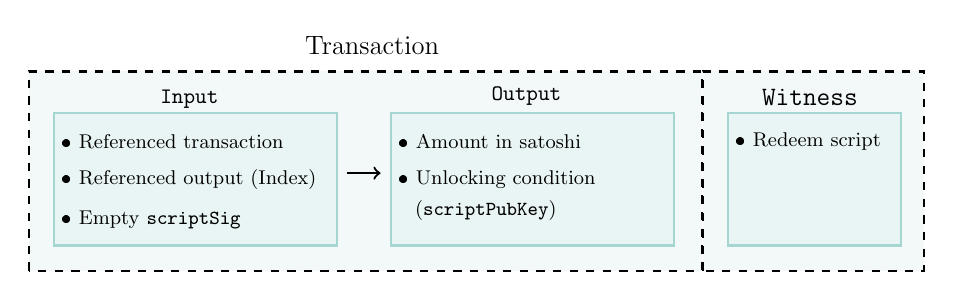
\begin{tikzpicture}[scale=0.8, every node/.style={scale=0.8}]
    
        \filldraw[yshift=-0.05cm, xshift=0.1cm,color = highlight!15, thick, draw=black, dashed] (-4,-4) rectangle ++(304pt,90pt) ;
        
        \filldraw[yshift=-0.05cm, xshift=0.1cm,color = highlight!25, thick, draw=highlight] (-3.6,-3.6) rectangle ++(128pt,60pt) ;
        
        \uncover<2->{
        
        \filldraw[yshift=-0.05cm, xshift=0.1cm,color = highlight!15, thick, draw=black, dashed] (6.7,-4) rectangle ++(100pt,90pt) ;

        
        \draw[color=black] plot (8.5,-1.55) node [above]
    {\large{{\alert{\texttt{Witness}}}}};
    
         \filldraw[yshift=-0.05cm, xshift=0.1cm,color = highlight!25, thick, draw=highlight] (7.1,-3.6) rectangle ++(78pt,60pt) ;
         
        \draw[color=black] plot (7.2,-2)   node[right] {\small{\textbullet{} {\alert{Redeem script}}}};
        
        }

    \draw[->,thick] (1.15,-2.5) -- (1.685,-2.5) ;
    
    \draw[color=black] plot (-1.35,-1.6)   node[above] {\texttt{Input}};
    \draw[color=black] plot (-3.5,-2)   node[right] {\small{\textbullet{} {Referenced transaction}}};
    \draw[color=black] plot (-3.5,-2.6)   node[right] {\small{\textbullet{} Referenced output (Index)}};
    \draw[color=black] plot (-3.5,-3.25)   node[right] {\small{\textbullet{} \alert{Empty \texttt{scriptSig}}}};
    \draw[color=black] plot (1.55,-0.2) node [below]
    {\large{{Transaction}}};
    
        \filldraw[yshift=-0.05cm, xshift=0.1cm,color = highlight!25, thick, draw=highlight] (1.75,-3.6) rectangle ++(128pt,60pt) ;
            
    \draw[color=black] plot (4,-1.55)   node[above] {\texttt{Output}};
    \draw[color=black] plot (1.85,-2)   node[right] {\small{\textbullet{} Amount in satoshi}};
    \draw[color=black] plot (1.85,-2.6)   node[right] {\small{\textbullet{} Unlocking condition}};
    \draw[color=black] plot (2,-3.1)   node[right] {\small{ (\texttt{scriptPubKey})}};
    
\end{tikzpicture}	
	\end{figure}
	\vspace{1em}
	
	\uncover<3->{$\rightarrow$ The \texttt{scriptSig} is always the same. The transaction's hash value is now an unambiguous transaction identifier.}
\end{frame}
%%%

%%%
\begin{frame}{Sort Fork Implementation}
		From the \href{https://cryptolectures.teachable.com/courses/bitcoin-blockchain-and-cryptoassets/lectures/30728731}{\link Fork Theory lecture}:\\
	\begin{figure}
		%%% Figure from: Schär, Fabian. "Blockchain Forks: A Formal Classification Framework and Persistency Analysis." (2020). 

\begin{table}[h!]
\center
  \begin{tabular}{ccc}
  \hline \hline
     & \scriptsize $S_{new}$ dominant ($r_{new}>r_{old}$) & \scriptsize $S_{old}$ dominant ($r_{new}<r_{old}$)\\ \cline{2-3}
     &&\\
    Soft fork & %($S_{new} \subset S_{old}$)&
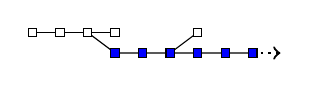
\begin{tikzpicture}[domain=1:10,scale=0.35, every node/.style={scale=0.35}]
\coordinate (o1) at (1,1);
\coordinate (o2) at (2,1);
\coordinate (o3) at (3,1);
\coordinate (o4) at (4,1);
\coordinate (o5) at (5,1);
\coordinate (o6) at (6,1);
\coordinate (o7) at (7,1);
\coordinate (o8) at (8,1);
\coordinate (o9) at (9,1);
\coordinate (o10) at (10,1);
\coordinate (n1) at (1,0.25);
\coordinate (n2) at (2,0.25);
\coordinate (n3) at (3,0.25);
\coordinate (n4) at (4,0.25);
\coordinate (n5) at (5,0.25);
\coordinate (n6) at (6,0.25);
\coordinate (n7) at (7,0.25);
\coordinate (n8) at (8,0.25);
\coordinate (n9) at (9,0.25);
\coordinate (n10) at (10,0.25);

  \draw[] (o1) to[] (o2) to[] (o3) to[] (o4);
  \draw[] (o3) to[] (n4) to[] (n5) to[] (n6) to[] (n7) to[] (n8) to[] (n9);
  \draw[color=black] (n6) to[] (o7);
  %\draw[color=black,densely dashed] (o4) to[] (o5);
  %\draw[color=black,densely dashed] (o7) to[] (o8);
  \draw[color=black,thick, dotted, ->] (n9) to[] (n10);

  %\filldraw[draw=black,fill=white] (o1) circle (5pt);
  %\filldraw[draw=black,fill=white] (o2) circle (5pt);
  %\filldraw[draw=black,fill=white] (o3) circle (5pt);
  %\filldraw[draw=black,fill=white] (o4) circle (5pt);
  %\filldraw[draw=black,fill=white] (o5) circle (5pt);
  %\filldraw[draw=black,fill=white] (o6) circle (5pt);
  %\filldraw[draw=black,fill=white] (o7) circle (5pt);
  %\filldraw[draw=black,fill=white] (o8) circle (5pt);
  %\filldraw[draw=black,fill=white] (o9) circle (5pt);
  \node (rect) at (o1) [fill=white,draw,minimum width=0.3cm,minimum height=0.3cm] {};
  \node (rect) at (o2) [fill=white,draw,minimum width=0.3cm,minimum height=0.3cm] {};
  \node (rect) at (o3) [fill=white,draw,minimum width=0.3cm,minimum height=0.3cm] {};
  \node (rect) at (o4) [fill=white,draw,minimum width=0.3cm,minimum height=0.3cm] {};
  %\node (rect) at (o5) [fill=white,draw,minimum width=0.3cm,minimum height=0.3cm] {};
  %\node (rect) at (o6) [fill=white,draw,minimum width=0.3cm,minimum height=0.3cm] {};
  \node (rect) at (o7) [fill=white,draw,minimum width=0.3cm,minimum height=0.3cm] {};
  %\node (rect) at (o8) [fill=white,draw,minimum width=0.3cm,minimum height=0.3cm] {};
  %\node (rect) at (o9) [fill=white,draw,minimum width=0.3cm,minimum height=0.3cm] {};
  %\filldraw[draw=black,fill=blue] (n4) circle (5pt);
  %\filldraw[draw=black,fill=blue] (n5) circle (5pt);
  %\filldraw[draw=black,fill=blue] (n6) circle (5pt);
  %\filldraw[draw=black,fill=blue] (n7) circle (5pt);
  %\filldraw[draw=black,fill=blue] (n8) circle (5pt);
  %\filldraw[draw=black,fill=blue] (n9) circle (5pt);
  %\node (rect) at (n1) [fill=white,draw,minimum width=0.3cm,minimum height=0.3cm] {};
  %\node (rect) at (n2) [fill=white,draw,minimum width=0.3cm,minimum height=0.3cm] {};
  %\node (rect) at (n3) [fill=white,draw,minimum width=0.3cm,minimum height=0.3cm] {};
  \node (rect) at (n4) [fill=blue,draw,minimum width=0.3cm,minimum height=0.3cm] {};
  \node (rect) at (n5) [fill=blue,draw,minimum width=0.3cm,minimum height=0.3cm] {};
  \node (rect) at (n6) [fill=blue,draw,minimum width=0.3cm,minimum height=0.3cm] {};
  \node (rect) at (n7) [fill=blue,draw,minimum width=0.3cm,minimum height=0.3cm] {};
  \node (rect) at (n8) [fill=blue,draw,minimum width=0.3cm,minimum height=0.3cm] {};
  \node (rect) at (n9) [fill=blue,draw,minimum width=0.3cm,minimum height=0.3cm] {};
\end{tikzpicture}
    &
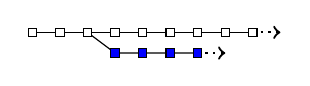
\begin{tikzpicture}[domain=1:10,scale=0.35, every node/.style={scale=0.35}]
\coordinate (o1) at (1,1);
\coordinate (o2) at (2,1);
\coordinate (o3) at (3,1);
\coordinate (o4) at (4,1);
\coordinate (o5) at (5,1);
\coordinate (o6) at (6,1);
\coordinate (o7) at (7,1);
\coordinate (o8) at (8,1);
\coordinate (o9) at (9,1);
\coordinate (o10) at (10,1);
\coordinate (n1) at (1,0.25);
\coordinate (n2) at (2,0.25);
\coordinate (n3) at (3,0.25);
\coordinate (n4) at (4,0.25);
\coordinate (n5) at (5,0.25);
\coordinate (n6) at (6,0.25);
\coordinate (n7) at (7,0.25);
\coordinate (n8) at (8,0.25);
\coordinate (n9) at (9,0.25);
\coordinate (n10) at (10,0.25);

  \draw[color=black] (o1) to[] (o2) to[] (o3) to[] (o4) to (o5) to (o6) to (o7) to (o8) to (o9);
  \draw[color=black] (o3) to[] (n4) to[] (n5) to[] (n6) to[] (n7);
  \draw[color=black,thick, dotted, ->] (o9) to[] (o10);
  \draw[color=black,thick, dotted, ->] (n7) to[] (n8);

  %\filldraw[draw=black,fill=white] (o1) circle (5pt);
  %\filldraw[draw=black,fill=white] (o2) circle (5pt);
  %\filldraw[draw=black,fill=white] (o3) circle (5pt);
  %\filldraw[draw=black,fill=white] (o4) circle (5pt);
  %\filldraw[draw=black,fill=white] (o5) circle (5pt);
  %\filldraw[draw=black,fill=white] (o6) circle (5pt);
  %\filldraw[draw=black,fill=white] (o7) circle (5pt);
  %\filldraw[draw=black,fill=white] (o8) circle (5pt);
  %\filldraw[draw=black,fill=white] (o9) circle (5pt);
  \node (rect) at (o1) [fill=white,draw,minimum width=0.3cm,minimum height=0.3cm] {};
  \node (rect) at (o2) [fill=white,draw,minimum width=0.3cm,minimum height=0.3cm] {};
  \node (rect) at (o3) [fill=white,draw,minimum width=0.3cm,minimum height=0.3cm] {};
  \node (rect) at (o4) [fill=white,draw,minimum width=0.3cm,minimum height=0.3cm] {};
  \node (rect) at (o5) [fill=white,draw,minimum width=0.3cm,minimum height=0.3cm] {};
  \node (rect) at (o6) [fill=white,draw,minimum width=0.3cm,minimum height=0.3cm] {};
  \node (rect) at (o7) [fill=white,draw,minimum width=0.3cm,minimum height=0.3cm] {};
  \node (rect) at (o8) [fill=white,draw,minimum width=0.3cm,minimum height=0.3cm] {};
  \node (rect) at (o9) [fill=white,draw,minimum width=0.3cm,minimum height=0.3cm] {};
  %\filldraw[draw=black,fill=blue] (n4) circle (5pt);
  %\filldraw[draw=black,fill=blue] (n5) circle (5pt);
  %\filldraw[draw=black,fill=blue] (n6) circle (5pt);
  %\filldraw[draw=black,fill=blue] (n7) circle (5pt);
  %\filldraw[draw=black,fill=blue] (n8) circle (5pt);
  %\filldraw[draw=black,fill=blue] (n9) circle (5pt);
  %\node (rect) at (n1) [fill=white,draw,minimum width=0.3cm,minimum height=0.3cm] {};
  %\node (rect) at (n2) [fill=white,draw,minimum width=0.3cm,minimum height=0.3cm] {};
  %\node (rect) at (n3) [fill=white,draw,minimum width=0.3cm,minimum height=0.3cm] {};
  \node (rect) at (n4) [fill=blue,draw,minimum width=0.3cm,minimum height=0.3cm] {};
  \node (rect) at (n5) [fill=blue,draw,minimum width=0.3cm,minimum height=0.3cm] {};
  \node (rect) at (n6) [fill=blue,draw,minimum width=0.3cm,minimum height=0.3cm] {};
  \node (rect) at (n7) [fill=blue,draw,minimum width=0.3cm,minimum height=0.3cm] {};
  %\node (rect) at (n8) [fill=white,draw,minimum width=0.3cm,minimum height=0.3cm] {};
  %\node (rect) at (n9) [fill=white,draw,minimum width=0.3cm,minimum height=0.3cm] {};
\end{tikzpicture}
\\
&&\\ \hline \hline
  \end{tabular}
\end{table}
	
	\end{figure}
	\vspace{1em}
	\begin{scriptsize}
	\uncover<2->{
		\textbf{If $r_{new} > r_{old}$:}\\
		\begin{itemize}
			\item \textbf{Nodes following $S_{old}$:} see SegWit transactions as \texttt{ANYONECANSPEND} and accept blocks with SegWit transactions
			\item \textbf{Nodes following $S_{new}$:} if \texttt{scriptSig} is empty $\rightarrow$ check \texttt{witness} for valid signature.
			\item The stricter rule set results in one dominant chain.
		\end{itemize}
	}
	\vspace{1em}
	\uncover<3->{
		\textbf{If $r_{new} < r_{old}$:}\\
		\begin{itemize}
			\item \textbf{Nodes following $S_{old}$:} consensus relevant nodes (CRNs) may create new blocks where they spend the \texttt{ANYONECANSPEND} outputs themselves.
			\item \textbf{Nodes following $S_{new}$:} check \texttt{witness} for valid signature and reject blocks where CRNs spend SegWit transactions themselves.
			\item Consensus conflict! Who can spend the output?
		\end{itemize}
	}
	\end{scriptsize}
\end{frame}
%%%

%%%
\begin{frame}{SegWit Transaction Types (P2WPKH)}
	Pay-to-witness-public-key-hash (P2WPKH) is the SegWit equivalent to P2PKH.\\
	\vspace{1.5em}
	
	\shadowbox{
		\begin{minipage}[c]{4.1in}
			\texttt{scriptSig:}\\
			\texttt{scriptPubKey:\ 0 <pubKeyHash>}\\
			\texttt{witness:\ <sig> <pubKey>}
		\end{minipage}
	}
	\vspace{1.5em}

	\textbf{Non-SegWit nodes:} output can be spent without the need for a signature.\\
	\vspace{0.5em}
	\textbf{SegWit nodes:} ''look for and verify the signature in the witness data."
\end{frame}
%%%

%%%
\begin{frame}{SegWit Transaction Types (P2WSH)}
	Pay-to-witness-script-has (P2WSH) is the SegWit equivalent to P2SH.\\
	\vspace{1.5em}
	
	\shadowbox{
		\begin{minipage}[c]{4.1in}
			\texttt{scriptSig:}\\
			\texttt{scriptPubKey:\ 0 <scriptHash256>}\\
			\texttt{witness:\ Any valid script}
		\end{minipage}
	}
	\vspace{1.5em}

	\textbf{Non-SegWit nodes:} output can be spent by anyone.\\
	\vspace{0.5em}
	\textbf{SegWit nodes:} ''look for and verify the script in the witness data."
\end{frame}
%%%

%%%
\begin{frame}{P2SH Embedded SegWit Transactions}

	\begin{figure}
		\begin{tikzpicture}
	\node[label = below:{Sender, $S_{old}$}] at (-4, 0) {
\includegraphics[height = 0.15\textheight]{../assets/images/agents/handing_right}};
	
	\node[label = below:{Receiver, $S_{new}$}] at (0, 0) {
\includegraphics[height = 0.15\textheight]{../assets/images/agents/reaching_left}};
	
	\draw[->, ultra thick] (-3.2, 0) -- (-0.8,0);
\end{tikzpicture}	
	\end{figure}
	\vspace{1.5em}
	
	\uncover<2->{
		$\rightarrow$ The receiver creates a P2SH Bitcoin address embedding the SegWit script in the P2SH locking condition:
	}
	\vspace{1em}
	
	\uncover<3->{
		\begin{itemize}
			\item P2SH: \texttt{OP\_HASH160 <scriptHash> OP\_EQUALVERIFY}
			\begin{itemize}
				\item<4-> P2SH(P2WPKH): \texttt{<scriptHash> = 0 <pubKeyHash>}
				\item<5-> P2SH(P2WSH): \texttt{<scriptHash> = 0 <scriptHash256>}
			\end{itemize}
		\end{itemize}
	}
	\end{frame}
%%%

%%%
\begin{frame}{Native SegWit Address (Bech32)}
	\begin{itemize}
%		\item Native SegWit address format
%		\item Always start with \texttt{bc1}
%		\item Encode SegWit outputs in an efficient and secure way
%		\item Case insensitivity
%		\item Stronger checksums: Bose-Chaudhuri-Hocquenghem SOURCE
		\item Consist of \texttt{bc1} prefix, version number, witness script and six-character checksum	
	\end{itemize}
	
	\vspace{1.5em}
	
	\begin{scriptsize}
		\texttt{$\overline{BC}_{pkh}$ = bc1qryqazre3142dvj8jrg8ed9s6t56aql6puy8wk8}\\
		\texttt{$BC_{sh}$ = bc1qrp33g0q5c5txsp9arysrx4k6zdkfs4nce4xj0gdcccefvpysxf3qccfmv3}
	\end{scriptsize}
\end{frame}
%%%

%%%
\begin{frame}{Confirmation Capacity Increase}
	\begin{scriptsize}
	$S_{old}$: blocks can only be 1MB large.\\
	$\rightarrow$ moving the redeem script to the witness field reduces the size of the transaction data that counts towards this limitation.\\
	\vspace{0.5em}
	\uncover<2->{
	$S_{new}$: blocks can only have a weight $W \leq 4$MB.\\}
		\begin{columns}[T]
			\begin{column}{0.5\textwidth}
				\uncover<3->{
					\begin{align*}
						W &= 3 \cdot (1 - \beta) bs(\texttt{all})\\
						&= bs(\texttt{all}) [3 \cdot (1 - \beta) + 1] \\
					\end{align*}
				}
			\end{column}
			\begin{column}{0.5\textwidth}
				\uncover<4->{
					\begin{align*}
						bs(\texttt{all}) &\leq \frac{4}{3 \cdot (1 - \beta) + 1}	
					\end{align*}
				}
			\end{column}
		\end{columns}
	\vspace{-3em}
		\uncover<5->{
			\begin{figure}
				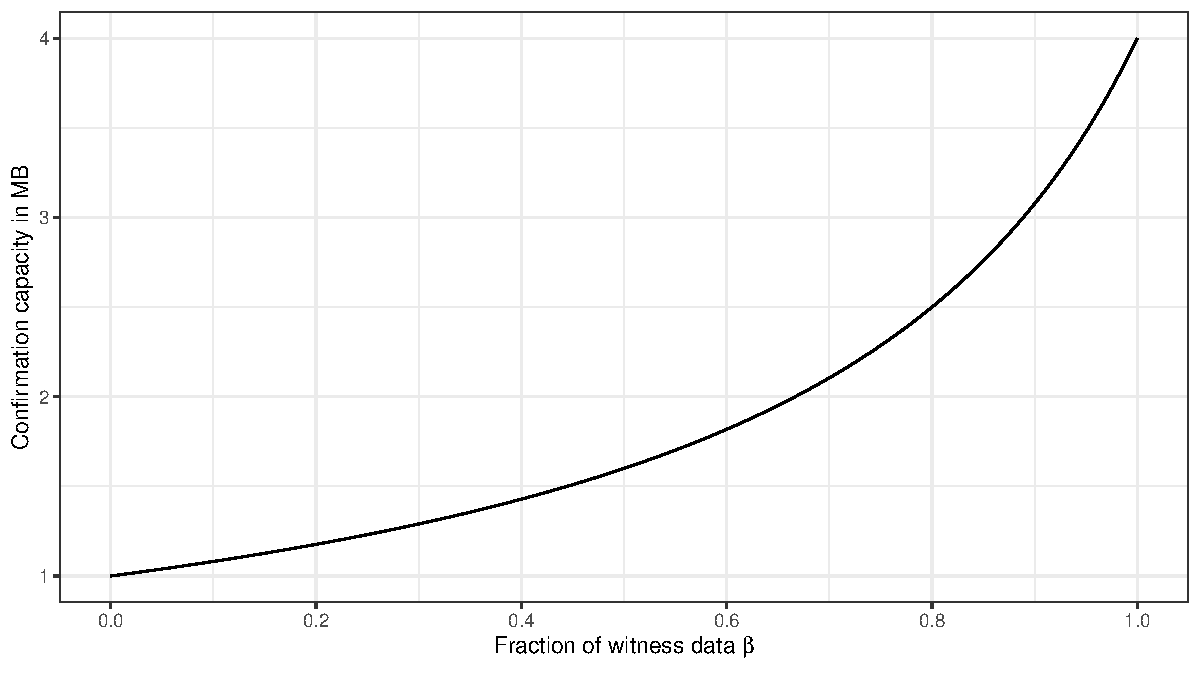
\includegraphics[width = 0.9\textwidth]{../assets/figures/confirmation-capacity-segwit.pdf}	
			\end{figure}
		}
	\end{scriptsize}
\end{frame}
%%%

%%%
%\begin{frame}%[allowframebreaks]
%\frametitle{References and Recommended Reading}
%	\bibliographystyle{amsplain}
%	\bibliography{../assets/bib/refs}
%\end{frame}
%%%

\end{document}